\documentclass{article}
\usepackage[utf8]{inputenc}
\usepackage{kpfonts}
\usepackage{commath}
\usepackage{amsthm}
\usepackage{graphicx}
\usepackage[margin=0.8in]{geometry}

\newcommand{\R}{\ensuremath{\mathbb{R}}}
\newcommand{\N}{\ensuremath{\mathbb{N}}}
\newcommand{\Q}{\ensuremath{\mathbb{Q}}}
\newcommand{\B}{\ensuremath{\mathcal{B}}}
\newcommand{\wrt}{with respect to}
\newcommand{\nbd}{neighborhood}
\newcommand{\Iff}{if and only if}
\newcommand{\ts}{topological space}
\newcommand{\es}{\ensuremath{\emptyset}}
\newcommand{\coleq}{\ensuremath{\coloneqq}}
\newcommand{\powset}[1]{\ensuremath{\mathcal{P}(#1)}}
\newcommand{\define}[1]{\textbf{\underline{#1}}}
\newcommand{\card}[1]{\ensuremath{\mathbf{card} (#1)}}
\newcommand{\func}[3]{\ensuremath{#1: #2 \to #3}}
\newcommand{\closure}[1]{\ensuremath{\overline{#1}}}
\newcommand{\ball}[3]{\ensuremath{B_{#1}^{#2}(#3)}}
\newcommand{\Ball}[3]{\ensuremath{\overline{B}_{#1}^{#2}(#3)}}
\newcommand{\fRR}{\ensuremath{f:\R \to \R}}
\newcommand{\tp}{\ensuremath{\mathcal{T}}}
\newcommand{\Ts}[2]{\ensuremath{(#1,#2)}}
\newcommand{\tpcof}{\ensuremath{\tp_\text{cof}}}
\newcommand{\tpdisc}{\ensuremath{\tp_\text{disc}}}
\newcommand{\tptriv}{\ensuremath{\tp_\text{triv}}}
\newcommand{\tpeuc}{\ensuremath{\tp_\text{Euc}}}
\newcommand{\Beuc}{\ensuremath{\B_\text{Euc}}}
\newcommand{\union}{\cup}
\newcommand{\Union}{\bigcup}
\newcommand{\inter}{\cap}
\newcommand{\Inter}{\bigcap}
\newcommand{\interior}[1]{\ensuremath{\mathring{#1}}}
\newcommand{\bound}[1]{\ensuremath{\partial #1}}
\renewcommand{\Subset}{\subseteq}
\renewcommand{\Supset}{\supseteq}

\theoremstyle{definition}
\newtheorem*{defn}{Definition}
\newtheorem*{cor}{Corollary}
\newtheorem*{thm}{Theorem}
\newtheorem*{prop}{Proposition}
\newtheorem*{ex}{Ex}
\newtheorem*{lem}{Lemma}

\theoremstyle{remark}
\newtheorem*{rmk}{Remark}

\begin{document}
    \begin{center}
        \textsc{Dillan Marroquin\\MATH 440.1001\\Scribing Week 6\\Due. 8 March 2021\\}
    \end{center}
        
    \noindent\section*{\textbf{\textsc{Lecture 15}}}{
        \subsection*{Continuous Functions and Homeomorphisms}
            \begin{defn}[15.1 Continuity]
            Let $\Ts{X}{\tp_X}, \, \Ts{Y}{\tp_Y}$ be topological spaces. Let $x \in X$. A function $\func{f}{X}{Y}$ is \define{continuous at $x$} \Iff{} for every open subset $V \Subset Y$ containing $f(x)$, there is an open subset $U \Subset X$ such that $x\in U$ and $f(U) \Subset V$. $\func{F}{X}{Y}$ is \define{continuous} \Iff{} $\forall x \in X$, $f$ is continuous at $x$.
        \end{defn}
        
        \begin{thm}[15.2]
            A function $\func{f}{X}{Y}$ is is continuous \Iff{} for every open subset $V \Subset Y$, $f^{-1}(Y) \Subset X$ is open.
        \end{thm}
        
        \begin{itemize}
            \item There exist many examples of maps between spaces\ldots
            \begin{itemize}
                \item Metric Spaces: Let $(X,d)$ be a metric space. Recall the definition of open balls: $\ball{x}{}{\varepsilon}\coleq \{x'\in X|d(x',x)<\varepsilon\}$.
                \item Define a basis for a topology $\B_d\coleq\{\ball{x}{}{\varepsilon}|x\in X, \, \varepsilon>0\}$.
                \item The topology $\tp_d$ generated by $\B_d$ is the metric topology and from Prop. 12.1, $\tp_d\coleq\{U \Subset X| \forall x\in U, \, \exists\varepsilon>0 \text{ such that }\ball{x}{}{\varepsilon} \Subset U\}$.
            \end{itemize}
        \end{itemize}
        
        \begin{prop}[15.3]
            Let $(X,d_X), \, (Y,d_Y)$ be metric spaces and $\tp_{d_X}, \, \tp_{d_Y}$ be their corresponding metric topologies. Then a function $\func{f}{X}{Y}$ is a map between $(X,d_X)$ and $(Y,d_Y)$ \Iff{} $\forall a \in X$ and $\forall \varepsilon > 0$, $\exists \delta_a > 0$ such that if $d_X(x,a) < \delta_a$, then $d_Y(f(x),f(a))<\varepsilon$.
        \end{prop}
        
        \begin{rmk}
            Prop. 15.3 implies that every continuous function $\func{f}{\R^n}{\R^m}$ from calculus is an example of a map between spaces!
        \end{rmk}
        }
        
    \noindent\section*{\textbf{\textsc{Lecture 16}}}{
        \begin{thm}[16.1]
            Let $\Ts{X}{\tp_X}, \, \Ts{Y}{\tp_Y}$ be topological spaces and let $\func{f}{X}{Y}$. Then
            \begin{enumerate}
                \item $f$ is continuous \Iff{} for every closed subset $B \Subset Y$, $f^{-1}(B) \Subset X$ is closed.
                \item Let $\B_X, \, \B_Y$ be bases for $\tp_X, \, \tp_Y$ respectively. Then $f$ is continuous \Iff{} $\forall B' \in \B_Y$ and $\forall x \in f^{-1}(B')$, $\exists B \Subset \B_X$ such that $x \in B \Subset f^{-1}(B')$.
            \end{enumerate}
        \end{thm}
        
        \begin{ex}[16.2 More Examples]\hfill
            \begin{enumerate}
                \item Let $\Ts{X}{\tp}$ be a space, $A \Subset X$ be any subset equipped with the subspace topology. Let $\func{i_A}{A}{X}$ be the "inclusion function" $i_A(a) \coleq a$. Then $i_A$ is continuous.\\
                Let $U \Subset X$ be open. Then $i^{-1}_A(U)=\{a\in A|a \in U\}$. Therefore, $U \inter A$ is open in $A$.
                \item Take above $A=X$. Then $i_X=\func{\mathrm{id}_X}{X}{X}$ is continuous.
                \item Constant maps: Let $X,Y$ be topological spaces with $y\in Y$ and define $\func{c_y}{X}{Y}, \, c_y(x)\coleq y \; \forall x\in X$. Then $c_y$ is continuous.
            \end{enumerate}
        \end{ex}
        
        \begin{prop}[16.3]
            If $\func{f}{X}{Y}, \, \func{g}{Y}{Z}$ are continuous functions between spaces $X, \, Y$ and $Z$, then $\func{g \circ f}{X}{Z}$ is continuous.
        \end{prop}
        
        \begin{cor}[16.4 Restriction of Domain]
            If $\func{f}{X}{Y}$ is continuous and $A \Subset X$ is equipped with the subspace topology, then the restriction $f|_A \coleq \func{f\circ i_A}{A}{Y}$ is continuous, where $i_A(a) \coleq a$.
        \end{cor}
        
        \begin{rmk}[16.5]
            Cor. 16.4 is simple yet useful!\\
            Let $S^2=\{(x,y,z)\in \R^3|x^2+y^2+z^2=1\}$ and let $\func{f}{S^2}{\R^2}$ be $f(x,y,z)\coleq(x^2-y^2,xz)$. Show $f$ is continuous.
            \begin{proof}
                Define $\func{\Bar{f}}{R^3}{R^2}$ to be $f(x,y,z)\coleq(x^2-y^2,xz)$. This is a continuous function by MATH 311, therefore by Cor. 16.4, $f=\Bar{f}\circ i_{S^2}$ is continuous.
            \end{proof}
        \end{rmk}
        
        \begin{prop}[16.6]
            Let $\func{f}{X}{Y}$ be continuous, $B \Subset Y$ be a subspace, and $\func{j_Y}{B}{Y}$ be the inclusion function. Suppose $f(X) \Subset B$. Then there exists a unique continuous function $\func{g}{X}{B}$ such that $f=j_B\circ g$.
        \end{prop}
        
        \begin{thm}[16.7 "Pasting Lemma"]
                Let $X,Y$ be topological spaces and let $\mathbf{a}=\{A_\alpha\}_{\alpha \in I}$ be a collection of subspaces of $X$ such that $X=\Union\limits_{\alpha\in I} A_\alpha$. Suppose $\{\func{f}{A_\alpha}{Y}\}_{\alpha \in I}$ is a collection of continuous functions such that $f_\alpha|_{A_\alpha \inter A_\beta} = f_\beta|_{A_\alpha \inter A_\beta} \; \forall \alpha,\beta \in I$. If either
                \begin{enumerate}
                    \item $\mathbf{a}$ is a collection of open subspaces of $X$, or
                    \item $\mathbf{a}$ is a finite collection of closed subspaces of $X$,
                \end{enumerate}
                then there exists a unique continuous function $\func{f}{X}{Y}$ such that $f|_{A_\alpha}=f_\alpha \; \forall \alpha\in I$.
        \end{thm}
    }
    \noindent\section*{\textbf{\textsc{Lecture 16}}}{
        We will begin by proving the Pasting Lemma from last lecture:
        
        \begin{proof}
            Let $\func{f}{X}{Y}$ be the set-theoretic function $f(x)\coleq f_\alpha (x)$ if $x\in A_\alpha$. Note that $f$ is well-defined \wrt{} the choice of $A_\alpha$: If $x \in A_\alpha \inter A_\beta$, then (1.) implies $f_\alpha(x)=f_\beta(x)$. Also note that if $\func{g}{X}{Y}$ is any function such that $g|_{A_\alpha}=f_\alpha \; \forall \alpha \in I$, then $f(x)=g(x) \; \forall x \in X$ which implies uniqueness. It remains to verify that $f$ is continuous:
            \indent \textbf{Case 1:} Let $V \Subset Y$ be open. Then 
            \begin{align*}
                f^{-1}(V)=f^{-1}(V) \inter X=f^{-1}(V) \inter \Union_{\alpha \in I} A_\alpha=\Union_{\alpha\in I}f^{-1}(V) \inter A_\alpha=\Union_{\alpha \in I}f^{-1}|_{A\alpha}(V)=\Union_{\alpha \in I}f^{-1}_\alpha(V).
            \end{align*}
            Since $\func{f_\alpha}{A_\alpha}{Y}$ is continuous by hypothesis, then $f_\alpha^{-1}(V) \Subset A_\alpha$ is open. By hypothesis, $A_\alpha \Subset X$ is open in $X$. PS2 \#1 implies $f_\alpha^{-1} (V) \Subset X$ is open subset of $X$. Therefore $\Union_{\alpha \in I}f^{-1}_\alpha(V)=f^{-1}(V)$ is open in $X$.\\
            \indent \textbf{Case 2:} This is an exercise on PS3 \#1. 
        \end{proof}
        \subsection*{Homeomorphisms: "Sameness" in Topology}
        
        \begin{defn}[17.1 Homeomorphism]
            A continuous injective and surjective function $\func{f}{X}{Y}$ between topological spaces is a \define{homeomorphism} \Iff{} its set-theoretic inverse $\func{f^{-1}}{Y}{X}$ is continuous.\\
            Two spaces are \define{homeomorphic} \Iff{} there exists a homeomorphism $\func{f}{X}{Y}$ between them. We write $X \cong Y$.
        \end{defn}
        
        \begin{rmk}[17.2] \hfill
            \begin{enumerate}
                \item $\forall X$ spaces, $\func{\mathrm{id}_X}{X}{X}$ is a homeomorphism.
                \item If $\func{f}{X}{Y}$ is a homeomorphism, then $\func{f^{-1}}{Y}{X}$ is also a homeomorphism.
                \item Given $X \xrightarrow{f} Y \xrightarrow{g} Z$, if $f$ and $g$ are homeomorphisms, then $\func{g\circ f}{X}{Z}$ is a homeomorphism.
            \end{enumerate}
            $\implies "X\cong Y$ is an equivalence relation "on the class of all topological spaces."
        \end{rmk}
        
        Note: It is NOT generally the case that if $\func{f}{X}{Y}$ is a continuous bijection of sets then $f$ is a homeomorphism.
        
        \begin{ex}\hfill
            \begin{enumerate}
                \item Let $\func{f}{(\R,\tpdisc)}{\R,\tptriv)}$ be the identity function $f(x)=x$.\\
                Claim: $f$ is continuous: $f^{-1}(\R)=\R, \; f^{-1}(\es)=\es$ and are open in any $\tp$ in $\R$. Therefore, $f$ is continuous.\\
                But $\func{f^{-1}}{(\R,\tptriv)}{(\R,\tpdisc)}$ is NOT continuous: $(f^{-1})^{-1}(\R-\{0\})=\R-\{0\}$ which is NOT open in $\Ts{\R}{\tptriv}$.
                \item Consider $\func{f}{[0,1)}{S^1}\coleq\{(x,y)\in\R|x^2+y^2=1\}$ with the subspace topology where $f(t)\coleq(\cos{2\pi t},\sin{2\pi t})$.\\
                Then $f$ is continuous (by Calculus) and is a bijection. Claim: $\func{f^{-1}}{S^1}{[0,1)}$ is NOT continuous.
                \begin{proof}
                    Observe $[0,1/2) \Subset [0,1)$ is an open subset of $[0,1)$. $(-1/2,1/2) \inter [0,1)=[0,1/2)$. We will show $W\coleq (f^{-1})^{-1}([0,1/2)) \Subset S^1$ is not open. Note $W=f([0,1/2))$ and $s_0=(1,0) \in W$.\\
                    For the sake of contradiction, suppose that $W \Subset S^1$ is an open subset of $S^1$. Then there exists an open subset $U \Subset R^2$ such that $W=S^1 \inter U \ni s_0$ and $s_0 \in U$. We know open balls form a basis for the topology on $\R^2$, which means $\exists \varepsilon > 0$ such that $\ball{s_0}{}{\varepsilon} \Subset U$ implies $\ball{s_0}{}{\varepsilon} \inter S^1 \Subset W$ (See diagram).
                    \begin{center}
                        \graphicspath{images}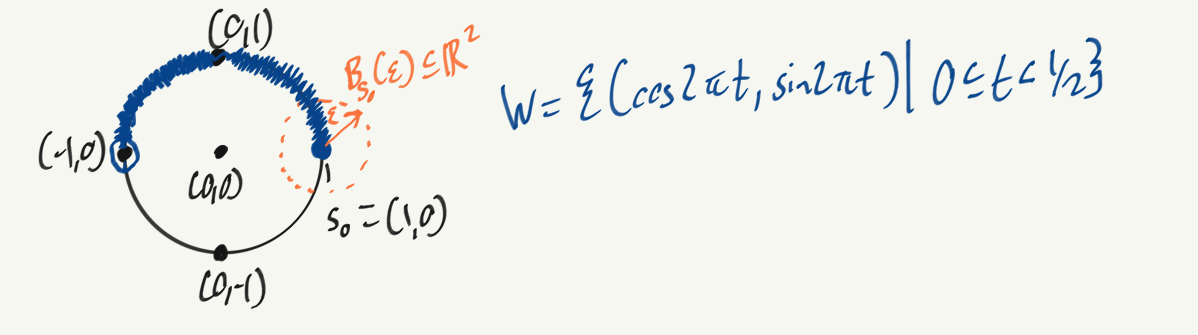
\includegraphics[scale = 0.25]{images/Proof Ex2.png}
                    \end{center}
                    But $\forall \varepsilon > 0$, there must be a point $(x,y) \in \ball{s_0}{}{\varepsilon} \inter S^1 \Subset W$ such that $y<0$. This is a contradiction since $\sin{2\pi t}\geq 0 \; \forall t\in [0,1/2)$. Hence no such $\varepsilon$ exists and therefore $W \Subset S^1$ is not open which implies $f^{-1}$ is not continuous, so $f$ is not a homeomorphism.
                \end{proof}
            \end{enumerate}
        \end{ex}
    }


        
\end{document}